\section{Цель работы}

Изучить использование логистической регрессии в качестве нейронной сети.

\section{Данные}

В работе предлагается использовать набор данных notMNIST, который состоит из изображений размерностью 28×28 первых 10 букв латинского алфавита (A … J, соответственно).
Обучающая выборка содержит порядка 500 тыс. изображений, а тестовая – около 19 тыс.


\section{Ход выполнения}

Для начала необходимо скачать набор данных notMNIST, который представляет из себя датасет букв латинского алфавита. За это отвечает функция prepare\_dataset:

\begin{lstlisting}
def prepare_dataset(url, save_as_name):
    """
    Prepares dataset to work with it
    :param url: url where resources is storing
    :param save_as_name: name of directory where it will be saved
    """
    if not os.path.exists(DATASETS_SOURCES_ROOT):
        logging.info("Dataset's source root doesn't exist, creating it...")
        os.mkdir(DATASETS_SOURCES_ROOT)

    if not os.path.exists(DATASETS_UNPACKED_ROOT):
        logging.info("Dataset's unpacking directory doesn't exist, creating it...")
        os.mkdir(DATASETS_UNPACKED_ROOT)

    logging.info("Start the dataset downloading...")
    sources_path = get_path_to_sources_dir(save_as_name)
    if os.path.exists(sources_path):
        logging.info("Dataset exists, downloading was ended...")
        return
    else:
        os.mkdir(sources_path)
        filename = fetch_dataset(url, sources_path)
        unpacked_path = get_path_to_unpacked_dir(save_as_name)
        unpack_dataset(filename, unpacked_path)
\end{lstlisting}

Отобразим данные из датасета:

\begin{figure}[h]
\centering
	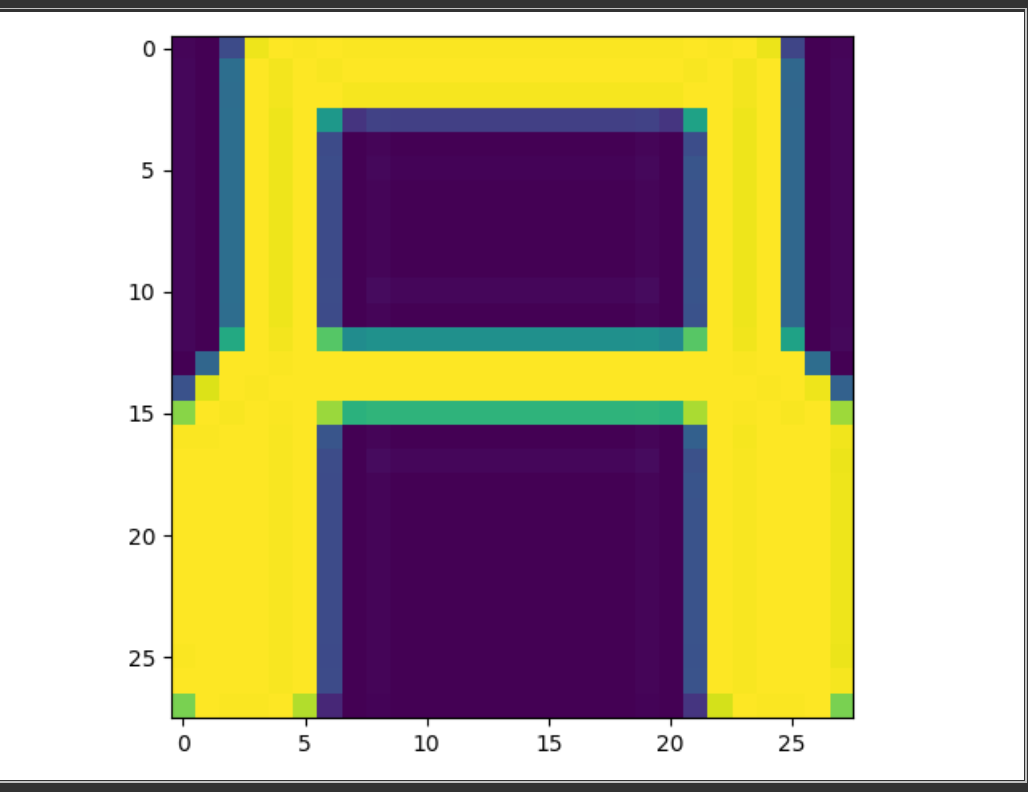
\includegraphics[totalheight=7cm]{a.png}
	\caption{Пример данных}
	\label{sec:purpose:payings}
\end{figure}

\begin{figure}[h]
\centering
	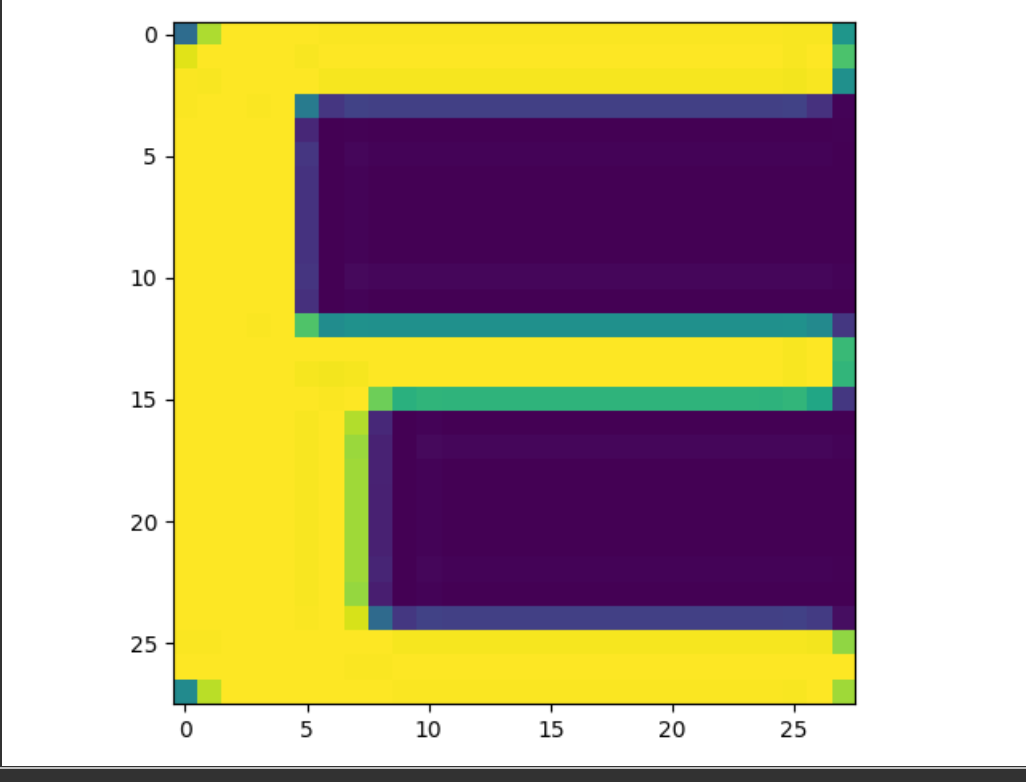
\includegraphics[totalheight=7cm]{e.png}
	\caption{Пример данных}
	\label{sec:purpose:payings}
\end{figure}

Далее сбалансируем данные, т.е. убедимся, что количество данных в каждом наборе примерно одинаково. Реализуем это через структуру данных Map:

\begin{lstlisting}
base = images_count[const.LEARNING_LETTERS[0]]
        for letter in const.LEARNING_LETTERS:
            if images_count[letter] - base > const.CLASSES_DIFFERENCE_ERROR:
                logging.error("Images have too much error!")
            logging.info("Classes have normal error. [letter s , elements s]", letter, images_count[letter])
\end{lstlisting}

Получим следующий вывод:

\begin{lstlisting}
2020-04-19 00:22:55,385: INFO --- root --- Classes have normal error. [letter A , elements 1872]
2020-04-19 00:22:55,385: INFO --- root --- Classes have normal error. [letter B , elements 1873]
2020-04-19 00:22:55,385: INFO --- root --- Classes have normal error. [letter C , elements 1873]
2020-04-19 00:22:55,385: INFO --- root --- Classes have normal error. [letter D , elements 1873]
2020-04-19 00:22:55,385: INFO --- root --- Classes have normal error. [letter E , elements 1873]
2020-04-19 00:22:55,385: INFO --- root --- Classes have normal error. [letter F , elements 1872]
2020-04-19 00:22:55,385: INFO --- root --- Classes have normal error. [letter G , elements 1872]
2020-04-19 00:22:55,385: INFO --- root --- Classes have normal error. [letter H , elements 1872]
2020-04-19 00:22:55,385: INFO --- root --- Classes have normal error. [letter I , elements 1872]
2020-04-19 00:22:55,385: INFO --- root --- Classes have normal error. [letter J , elements 1872]
\end{lstlisting}

Далее, разделим датасет на выборки - обучающую, валидационную и тестовую:

\begin{lstlisting}
        training_set = []
        validation_set = []
        test_set = []

        logging.info("Start sorting into sets")
        for letter in const.LEARNING_LETTERS:
            path_to_img_dir = get_path_to_unpacked_dir(usable_dataset_name) \
                              + "/" \
                              + usable_dataset_name \
                              + "/" \
                              + letter
            files_in_dir = list(map(lambda path: path_to_img_dir + "/" + path, os.listdir(path_to_img_dir)))
            files_count = len(files_in_dir)
            # calculate how many pics are going to each set
            to_training = int(files_count * const.TRAIN_SET_PERCENTS)
            to_validation = int(files_count * const.VALIDATION_SET_PERCENTS)
            to_test = files_count - to_training - to_validation
            # using slice put file paths to sets
            training_set = training_set + files_in_dir[0: to_training - 1]
            validation_set = validation_set + files_in_dir[to_training: to_training + to_validation - 1]
            test_set = test_set + files_in_dir[to_training + to_validation: to_training + to_validation + to_test - 1]


        logging.info(
            "Total set was separted to 3 sets: training (%d - %d %%), validation (%d - %d %%) and test (%d - %d %%)",
            len(training_set), const.TRAIN_SET_PERCENTS * 100,
            len(validation_set), const.VALIDATION_SET_PERCENTS * 100,
            len(test_set), const.TEST_SET_PERCENTS * 100
        )
\end{lstlisting}

Избавимся от дубликатов в выборках:

\begin{lstlisting}
        uniq_images = {}
        duplicate_images = {}
        logging.info("Start deleting duplicates...")
        for letter in const.LEARNING_LETTERS:
            path_to_img_dir = get_path_to_unpacked_dir(usable_dataset_name) \
                              + "/" \
                              + usable_dataset_name \
                              + "/" \
                              + letter
            files_in_dir = os.listdir(path_to_img_dir)
            for file in files_in_dir:
                full_path = path_to_img_dir + "/" + file
                hash = calc_file_hash(full_path)
                if hash not in uniq_images:
                    uniq_images[hash] = full_path
                else:
                    duplicate_images[hash] = full_path

        logging.info("Was found d duplicate images, total count of unique images = d", len(duplicate_images),
                     len(uniq_images))

        logging.info("Delete duplicated images from the sets")
        for non_uniq_hash in duplicate_images:
            non_uniq_path = duplicate_images[non_uniq_hash]
            if non_uniq_path in training_set:
                training_set.remove(non_uniq_path)
            if non_uniq_path in validation_set:
                validation_set.remove(non_uniq_path)
            if non_uniq_path in test_set:
                test_set.remove(non_uniq_path)

        logging.info(
            "Total count of sets after duplicate deleting: training: d ; validation: d ; test: d",
            len(training_set),
            len(validation_set),
            len(test_set)
        )
\end{lstlisting}

Увидим следующий вывод:

\begin{lstlisting}
2020-04-19 00:22:55,433: INFO --- root --- Total set was separted to 3 sets: training (11220 - 60 %), validation (3730 - 20 %) and test (3744 - 20 %)
2020-04-19 00:22:55,433: INFO --- root --- Start deleting duplicates...
2020-04-19 00:23:05,754: INFO --- root --- Was found 236 duplicate images, total count of unique images = 18232
2020-04-19 00:23:05,754: INFO --- root --- Delete duplicated images from the sets
2020-04-19 00:23:05,819: INFO --- root --- Total count of sets after duplicate deleting: training: 11150 ; validation: 3670 ; test: 3638
\end{lstlisting}

Далее натренируем логистическую регресси на выборках, для этого будем использовать библиотеку SkLearn. Обучение модели на n примерах описано в функции train\_on\_n\_examples:

\begin{lstlisting}
    def train_on_n_examples(self, x_train, x_test, y_train, y_test):
        train_examples_count = x_train.shape[1]
        test_examples_count = x_test.shape[1]
        logistic_regression = LogisticRegression(max_iter=1000, tol=1e-2, C=0.5, solver='liblinear',
                                                 penalty='l1')  # 1 mln
        logistic_regression.fit(x_train.T, y_train)
        logging.info("Model has been trained successfully!")

        score_result = logistic_regression.score(x_test.T, y_test)
        score_result_2 = logistic_regression.score(x_train.T, y_train)
        logging.info("Train examples count: d", train_examples_count)
        logging.info("Test examples count: d", test_examples_count)
        logging.info("Score on test data: f", score_result)
        logging.info("Score on train data: f", score_result_2)
        return (train_examples_count, score_result)
\end{lstlisting}

Результат выполнения обучения будет выведен в консоль:

\begin{lstlisting}
2020-04-19 00:23:08,747: INFO --- root --- Train examples count: 50
2020-04-19 00:23:08,747: INFO --- root --- Test examples count: 3638
2020-04-19 00:23:08,747: INFO --- root --- Score on test data: 0.619571
2020-04-19 00:23:08,747: INFO --- root --- Score on train data: 1.000000
2020-04-19 00:23:08,768: INFO --- root --- Model has been trained successfully!
2020-04-19 00:23:08,782: INFO --- root --- Train examples count: 100
2020-04-19 00:23:08,782: INFO --- root --- Test examples count: 3638
2020-04-19 00:23:08,782: INFO --- root --- Score on test data: 0.728422
2020-04-19 00:23:08,782: INFO --- root --- Score on train data: 1.000000
2020-04-19 00:23:09,086: INFO --- root --- Model has been trained successfully!
2020-04-19 00:23:09,105: INFO --- root --- Train examples count: 1000
2020-04-19 00:23:09,105: INFO --- root --- Test examples count: 3638
2020-04-19 00:23:09,105: INFO --- root --- Score on test data: 0.841396
2020-04-19 00:23:09,105: INFO --- root --- Score on train data: 1.000000
2020-04-19 00:23:11,881: INFO --- root --- Model has been trained successfully!
2020-04-19 00:23:11,944: INFO --- root --- Train examples count: 11150
2020-04-19 00:23:11,944: INFO --- root --- Test examples count: 3638
2020-04-19 00:23:11,944: INFO --- root --- Score on test data: 0.884827
2020-04-19 00:23:11,944: INFO --- root --- Score on train data: 0.924574
\end{lstlisting}

Продемонстрируем это на графике:

\begin{figure}[h]
\centering
	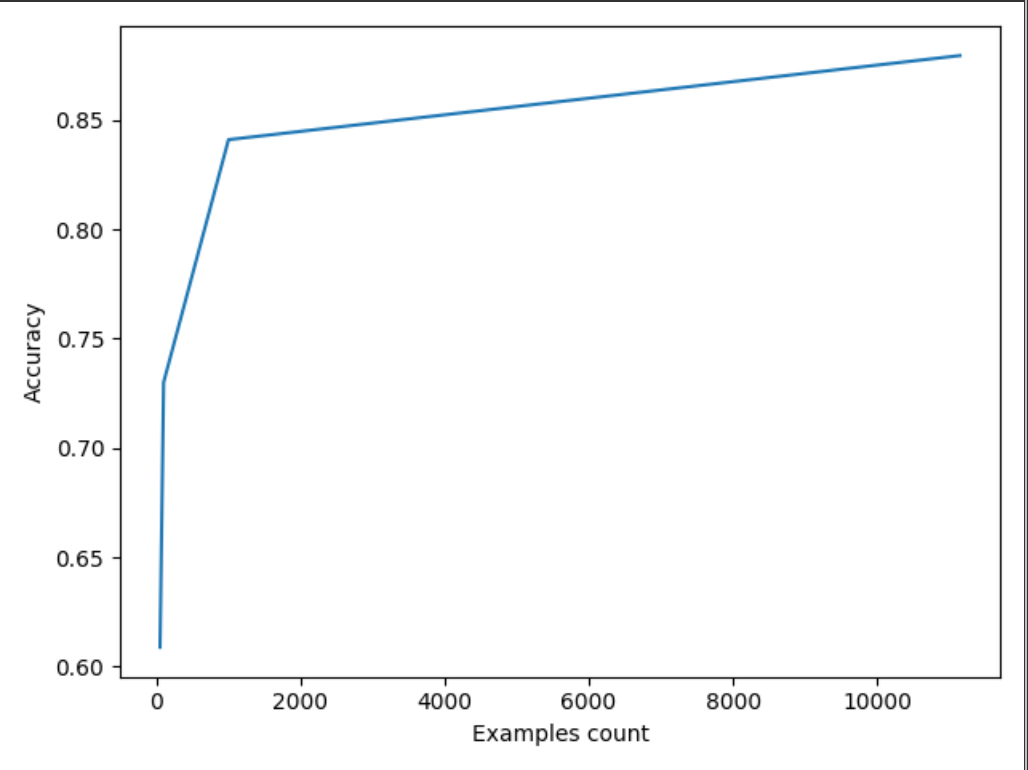
\includegraphics[totalheight=7cm]{graph.png}
	\caption{График обучения}
	\label{sec:purpose:payings}
\end{figure}

% \section{Цель работы}

% Целью данной лабораторной работы является создания решения в Hyperledger Composer. В результате должно получится полноценная сеть с развёрнутым API и подключённым к нему клиентом, способным взаимодействовать с сетью.

% \section{Ход выполнения работы}

% Первым этапом выполнения является установка всех необходимых компонентов, с помощью которых будет производится работа.

% К ним относятся:

% \begin{itemize}
% 	\item docker;
% 	\item docker-compose;
% 	\item nodejs;
% 	\item composer-cli;
% 	\item composer-rest-service;
% 	\item yo;
% 	\item composer-playground.
% \end{itemize}

% Предварительно установив все данные инструменты можно приступать непосредственно к разработке. Первым этапом является создание каркаса приложения при помощи инструмента Yeoman. Необходимо выполнить следующую команду.

% \begin{lstlisting}
% yo hyperledger-composer:businessnetwork
% \end{lstlisting}

% Во время её выполнения будет запрошены параметры создания - имя автора, лицензия, емейл и т.д.

% Следующим этапом является определение бизнес-сети. Бизнес-сеть состоит из активов, участников, транзакций, правил контроля доступа, а также необязательных событий и запросов. В скелетной бизнес-сети, созданной на предыдущих этапах, есть файл модели (.cto), который будет содержать определения классов для всех активов, участников и транзакций в бизнес-сети. Скелетная бизнес-сеть также содержит документ управления доступом (permissions.acl) с основными правилами контроля доступа, файл сценария (logic.js), содержащий функции процессора транзакций, и файл package.json, содержащий метаданные бизнес-сети.

% Определим модель как:

% \begin{lstlisting}
% namespace by.bsuir.tbch

% asset Computer identified by tradingSymbol {
%     o String tradingSymbol
%     o String description
%     o String mainExchange
%     o Double count
%     --> Seller seller
% }

% participant Seller identified by tradeId {
%     o String tradeId
%     o String firstName
%     o String lastName
%     o String name
% }

% transaction Trade {
%     --> Computer computer
%     --> Seller newSeller
% }
% \end{lstlisting}

% Даллее добавим логику транзакций на JavaScript:

% \begin{lstlisting}
% /**
%  * Track the trade of a computer from one trader to another
%  * @param {by.bsuir.tbch.Trade} trade - the trade to be processed
%  * @transaction
%  */
% async function tradeComputer(trade) {
%     trade.computer.seller = trade.newSeller;
%     let assetRegistry = await getAssetRegistry('by.bsuir.tbch.Computer');
%     await assetRegistry.update(trade.computer);
% }
% \end{lstlisting}

% Далее определим настройки доступа:

% \begin{lstlisting}
% /**
%  * Access control rules for tutorial-network
%  */
% rule Default {
%     description: "Allow all participants access to all resources"
%     participant: "ANY"
%     operation: ALL
%     resource: "by.bsuir.tbch.*"
%     action: ALLOW
% }

% rule SystemACL {
%   description:  "System ACL to permit all access"
%   participant: "ANY"
%   operation: ALL
%   resource: "org.hyperledger.composer.system.**"
%   action: ALLOW
% }
% \end{lstlisting}

% После настройки модели, обработчика и доступа необходимо создать архив бизнес сети с форматом .bna. Делается это следующей командой:

% \begin{lstlisting}
% composer archive create -t dir -n .
% \end{lstlisting}

% После создания файла .bna бизнес-сеть можно развернуть на экземпляре Hyperledger Fabric. Как правило, информация от администратора Fabric необходима для создания идентификатора PeerAdmin с привилегиями для установки кода цепи на одноранговый узел, а также для запуска кода цепи в канале композитного канала. Однако, как часть установки среды разработки, идентичность PeerAdmin уже создана.

% После того, как бизнес-сеть была установлена, сеть может быть запущена. Для лучшей практики следует создать новый идентификатор для администрирования бизнес-сети после развертывания.

% Далее необходимо задеплоить бизнес-сеть. Развертывание бизнес-сети в Hyperledger Fabric требует, чтобы бизнес-сеть Hyperledger Composer была установлена на одноранговом узле, затем можно запустить бизнес-сеть и создать нового участника, удостоверение и связанную карту, чтобы стать администратором сети. Наконец, бизнес-сетевая карта администратора сети должна быть импортирована для использования, и сеть может затем пропинговать, чтобы проверить, отвечает ли она.

% Для установки бизнес-сети необходимо запустить следующую команду:

% \begin{lstlisting}
% composer network install --card PeerAdmin@hlfv1 --archiveFile tutorial-network@0.0.1.bna
% \end{lstlisting}

% Для запуска установленной сети используется следующая команда:

% \begin{lstlisting}
% composer network start --networkName tutorial-network --networkVersion 0.0.1 --networkAdmin admin --networkAdminEnrollSecret adminpw --card PeerAdmin@hlfv1 --file networkadmin.card
% \end{lstlisting}

% Чтобы заимпортить сущность администратора необходимо запустить следующую команду:

% \begin{lstlisting}
% composer card import --file networkadmin.card
% \end{lstlisting}

% Далее проверим, всё ли работает после установки:

% \begin{lstlisting}
% composer network ping --card admin@tutorial-network
% \end{lstlisting}

% Hyperledger Composer может генерировать индивидуальный REST API на основе бизнес-сети. Для разработки веб-приложения REST API предоставляет полезный уровень нейтральной для языка абстракции.

% Для создания REST API на основе бизнес-сети используется следующая команда:

% \begin{lstlisting}
% composer-rest-server
% \end{lstlisting}

% Сгенерированный API подключен к развернутой цепочке блоков и бизнес-сети.

% Hyperledger Composer также может генерировать приложение Angular 4, работающее с REST API. Для этого используется следующая команда:

% \begin{lstlisting}
% yo hyperledger-composer:angular
% \end{lstlisting}

% \begin{figure}[h]
% \centering
% 	\includegraphics[totalheight=7cm]{1.png}
% 	\caption{Этапы создания бизнес-сети}
% 	\label{sec:purpose:payings}
% \end{figure}

% \begin{figure}[h]
% \centering
% 	\includegraphics[totalheight=7cm]{2.png}
% 	\caption{Окно создания транзакции}
% 	\label{sec:purpose:payings}
% \end{figure}

% \begin{figure}[h]
% \centering
% 	\includegraphics[totalheight=7cm]{3.png}
% 	\caption{Окно выполнения}
% 	\label{sec:purpose:payings}
% \end{figure}

% \begin{figure}[h]
% \centering
% 	\includegraphics[totalheight=7cm]{4.png}
% 	\caption{Участники}
% 	\label{sec:purpose:payings}
% \end{figure}

% \begin{figure}[h]
% \centering
% 	\includegraphics[totalheight=7cm]{5.png}
% 	\caption{Компьютеры}
% 	\label{sec:purpose:payings}
% \end{figure}

% \begin{figure}[h]
% \centering
% 	\includegraphics[totalheight=7cm]{6.png}
% 	\caption{Пример сгенерированного API}
% 	\label{sec:purpose:payings}
% \end{figure}

% \begin{figure}[h]
% \centering
% 	\includegraphics[totalheight=7cm]{7.png}
% 	\caption{Лист API эндпоинтов}
% 	\label{sec:purpose:payings}
% \end{figure}

% \section{Вывод}

% В результате выполнения лабораторной работы было создано решение при помощи Hyperledger Composer. Результат выполнения лабораторной работы был представлен в вышеописанном разделе.

% % \section{Задача прогнозирования временных рядов}
% % \label{sec:purpose}

% % Прогнозирование временных рядов является одним из важных факторов предсказания будущих значений, анализе трендов, циклов и сезонностей в определённых
% % значениях. Для начала, следует рассмотреть само понятие временного ряда.

% % Временной ряд: \begin{equation}\label{timeline_value} Y_1, Y_2 ... Y_t \in \mathbf{R}  \end{equation}, значения признака, измеренные через постоянные временные интервалы \cite{wiki}.

% % Ключевая особенность состоит в том, что измерения признака происходит во времени и между разными измерениями всегда проходит одинаковое количество времени.
% % Т.к. если промежуток между отсчётами будет случайным, то в этом случае это будет являться случайным процессом и методы для обработки будут использоваться другие, нежели
% % при работе с прогнозированием временных рядов.

% % В данном случае, мы рассматриваем прогнозирование вещественного скалярного ряда, т.е. измерения принадлежат множеству вещественных чисел ($R$).

% % Как простой пример временного ряда можно рассмотреть временной ряд заработных плат \cite{datamining_in_action}.

% % \begin{figure}[h]
% % \centering
% % 	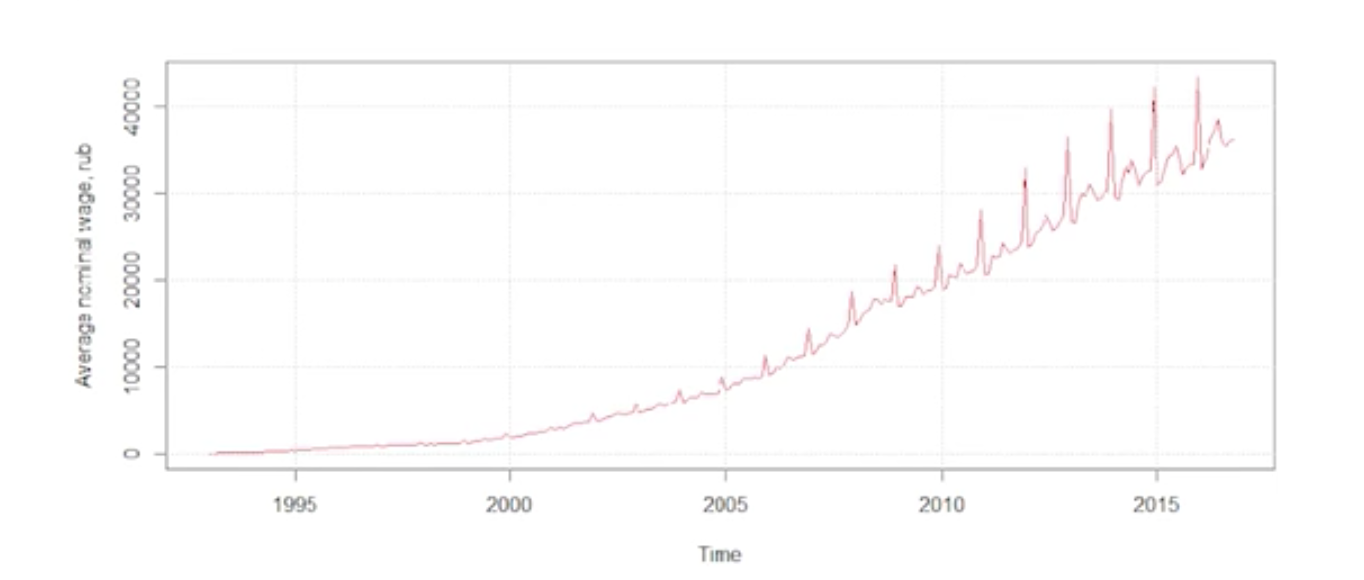
\includegraphics[totalheight=7cm]{main_part/timeline-payings.png}
% % 	\caption{Пример временного ряда}
% % 	\label{sec:purpose:payings}
% % \end{figure}

% % На данном рисунке видно, что, есть тренд к росту зарплат и пики, в декабре - месяце, где выдаются годовые премии. Длина ряда не является фиксированной величиной и может меняться, день, неделя, месяц, квартал, год. Сам по себе промежуток не имеет значения при прогнозировании.

% % Задачей прогнозирования временных рядов является поиск функции F, которая будет будет зависеть от всей известной информации к моменту прогнозирования, который обозначается $ T $. На вход данная функция принимает все значения ряда, от $ Y_1$ до $ Y_t $. Также, функция принимает дополнительный параметр $ H $, который показывает насколько вперёд необходимо прогнозировать ряд. Параметр $h$ принимает значения от 1 до $ H $ ($ h \in {1, 2, ... H} $), где $ H $ называется горизонтом прогнозирования.

% % Помимо прогнозов, которые представляют собой число, при прогнозировании полезно добавлять интервал, который показывает вероятность, с которой будет выполнено предсказание.
% % Такой интервал называется предсказательным. 

% % Предсказательный интервал - интервал, в котором предсказываемая величина окажется с вероятностью не меньше заданной. В данном случае, не стоит его путать с доверительным интервалом, который является случайным интервалом, для фиксированного неслучайного параметра. Предсказательный интервал является очень полезным инструментом, т.к. он показывает заказчику прогноза, насколько можно быть уверенным в произведённом прогнозе. И в данном случае важно, данную степень неуверенности квантифицировать.

% % Как пример: в апреле 1997 в городе Гранд-Фокс, Северная Дакота, произошло наводнение. Город был защищён дамбой высотой 51 фут, согласно прогнозу, высота паводка должна была составить 49 футов, истинная же высота, оказалась 54. В результате этой ошибки было эвакуировано 75\% населения города и нанесён ущерб на несколько миллиардов долларов. На исторических данных, точность прогнозов метеорологической службы составляла +- 9 футов.

% % Таким образом, выделим особенности задачи прогнозирования временных рядов:
% % \begin{itemize}
% % 	\item в классических задачах анализа данных предполагается независимость наблюдений;
% % 	\item при прогнозировании временных рядов, прогноз строится на исторических данных.
% % \end{itemize}

% % В отличии от задач машинного обучения и статистики, где значения, как правило, являются простой выборкой, т.е. разные наблюдения, померенные на разных объектах, независимые одинаково распределённые. В то время как при прогнозировании временных рядов, данные устроены принципиально по другому - будущее зависит от прошлого, т.е. чем меньше прошлое похоже на шум, тем точнее можно будет сделать прогноз.

% % Лучше всего, в машинном обучении, решаются задачи с учителем, т.е. есть определённом количество признаков и выходы, для данных признаков. В данном же случае, прогнозирования временных рядов, отсутсвуют $ x $-ы, т.е. отсутствуют признаки, есть только $y$-ки \cite{datamining_in_action}.

% % \begin{figure}[h]
% % \centering
% % 	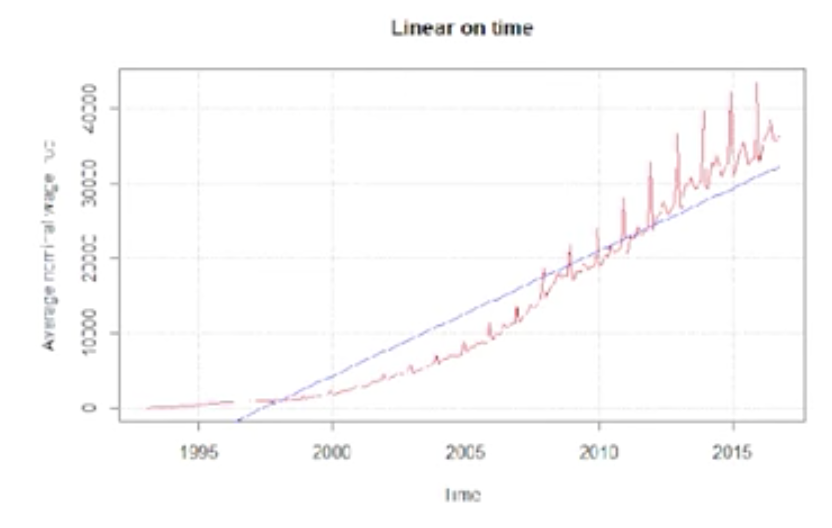
\includegraphics[totalheight=7cm]{main_part/linear-on-time.png}
% % 	\caption{Применение методов машинного обучения (линейное)}
% % 	\label{sec:purpose:linear}
% % \end{figure}

% % В данном рисунке видно, что предсказания (синяя линия) не будут достаточно точными, т.к. они явно не учитывают нешумовые всплески \cite{datamining_in_action}.

% % \begin{figure}[h]
% % \centering
% % 	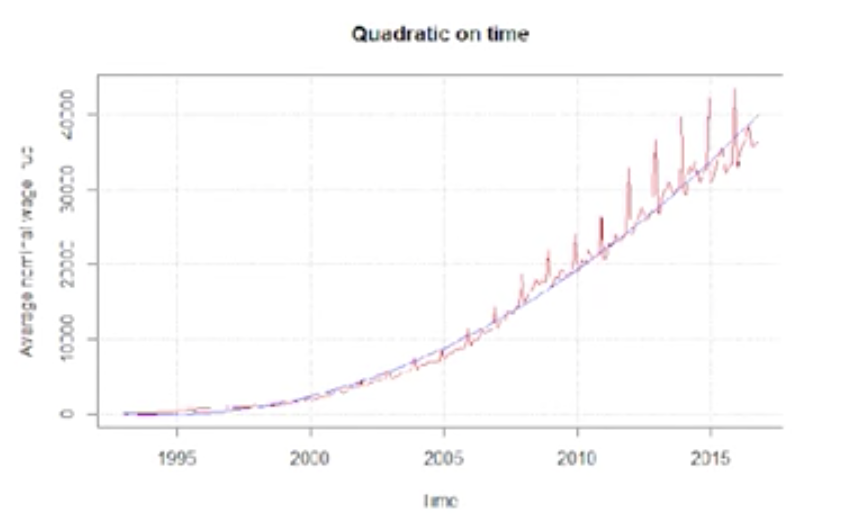
\includegraphics[totalheight=7cm]{main_part/quadratic-on-time.png}
% % 	\caption{Применение методов машинного обучения (квадратичное)}
% % 	\label{sec:purpose:quadratic}
% % \end{figure}

% % Также и применение квадратичной функции не приводит к точному предсказанию.

% % Ключевая особенность временного ряда заключается в том, что соседние значения не независимы. Квантифицировать это можно с помощью автокорреляции. Автокорреляция, это корреляция ряда с самим собой, сдвинутым на определённое количество отсчётов. То количество, на которое мы сдвигаем отсчёт, называется \textit{лагом} автокорреляции. Автокорреляция меняет свои значения от -1 до 1, 1 означает идеальную линейную зависимость с положительным знаком, -1 - линейная зависимость с отрицательным, 0 - отсутствие линейной зависимости.

% % Также необходимо рассмотреть компоненты временных рядов, т.е. то, из чего состоят ряды.

% % \textit{Тренд} - плавное долгосрочное среднего изменения уровня ряда. Ряд может <<колебаться>> вокруг своего тренда.

% % \textit{Сезонность} - циклические изменения уровня ряда с постоянным периодом. Например, если рассматриваются месячные ряды, то в них, скорее всего, будет годовая сезонность, т.е. то, что происходит в декабре этого года, будет похоже на то, что происходило в декабре предыдущего года.

% % \textit{Цикл} - изменения уровня ряда с переменным периодом (например экономические циклы, периоды солнечной активности).

% % \textit{Ошибка} - непрогнозируемая случайная компонента ряда.

% % Ошибку, также, можно описать как то, что нельзя описать любыми другими компонентами ряда. Рассмотрим несколько примеров.

% % В данном ряде можно рассмотреть тренд к падению количества контрактов сокровищницы США по дням \cite{datamining_in_action}.

% % \begin{figure}[h]
% % \centering
% % 	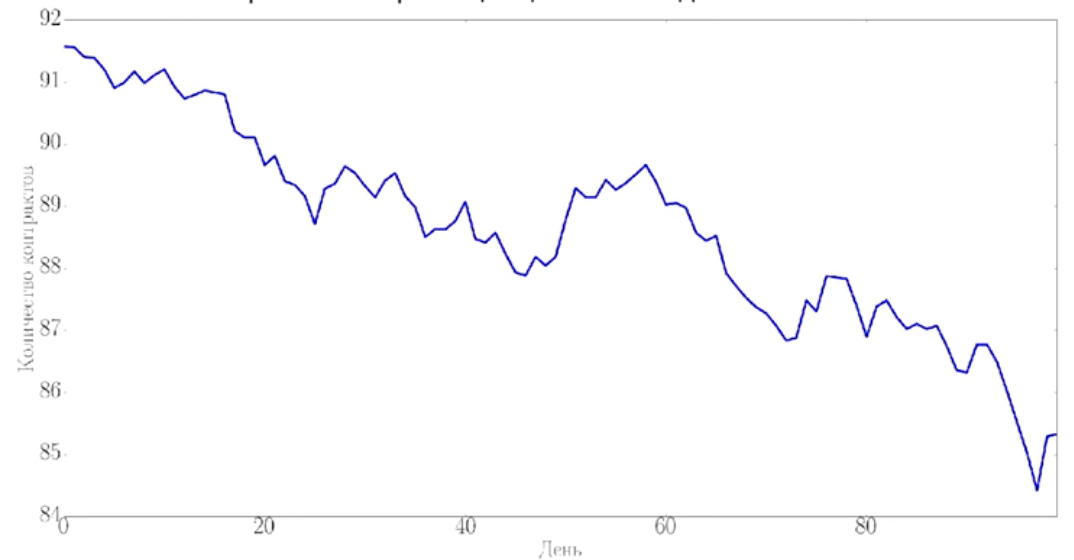
\includegraphics[totalheight=7cm]{main_part/usa-gold.png}
% % 	\caption{Количества контрактов сокровищницы США}
% % 	\label{sec:purpose:contracts}
% % \end{figure}

% % Это ряд, в котором можно отметить линейно понижающийся тренд. Можно сказать, что ряд совершает <<колебания>> вокруг своей линии тренда.

% % Далее можно рассмотреть ряд с объёмами производства электричества в Австралии \cite{datamining_in_action}.

% % \begin{figure}[h]
% % \centering
% % 	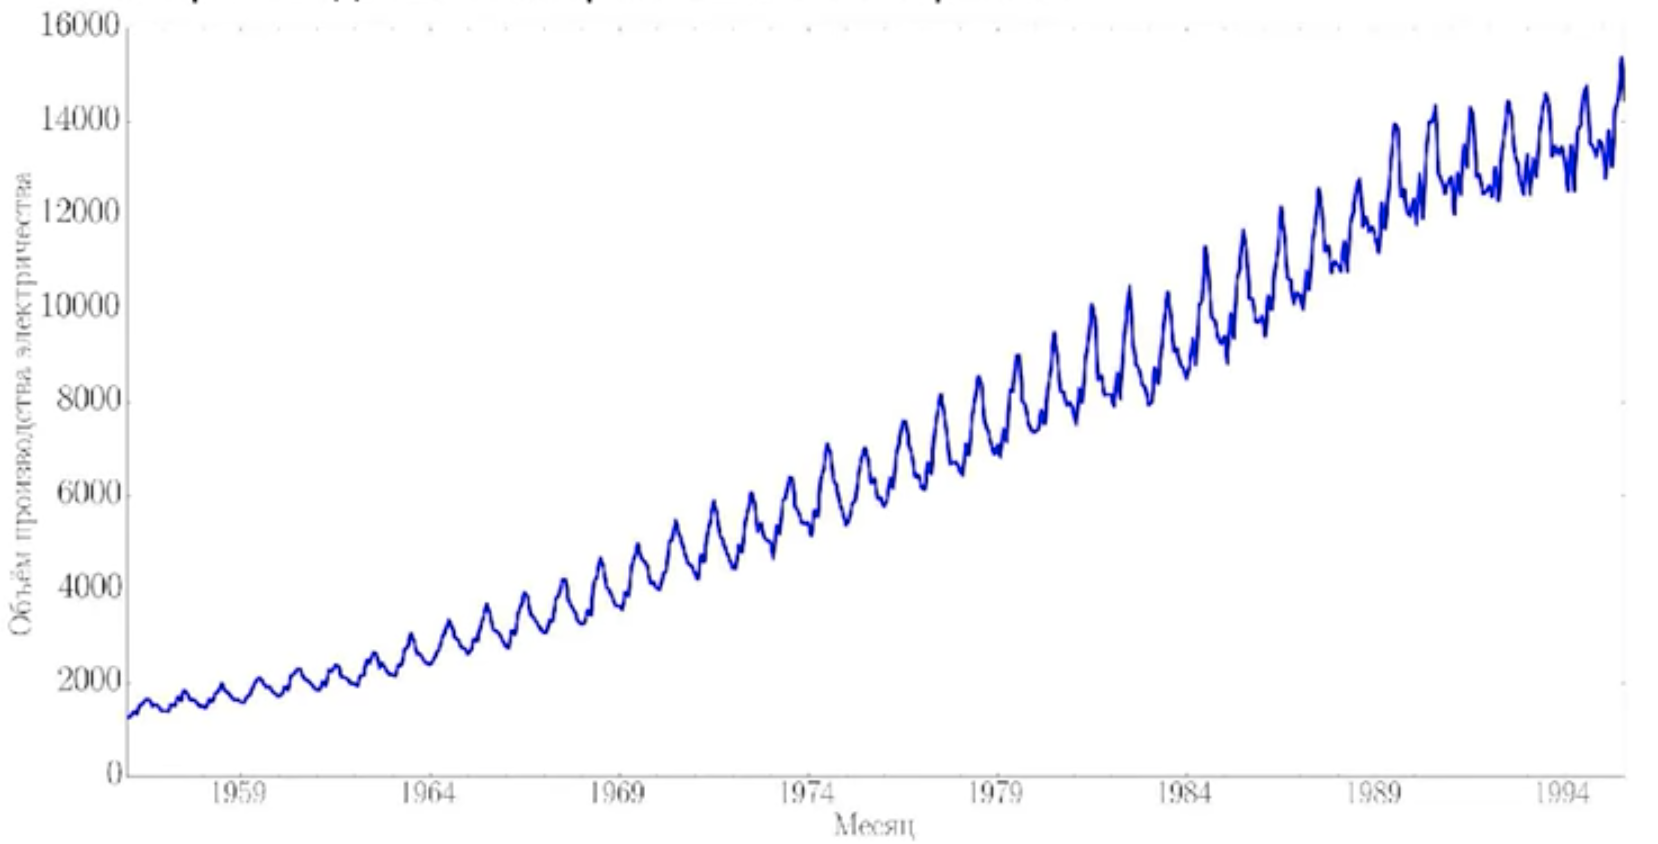
\includegraphics[totalheight=7cm]{main_part/australia-electricity.png}
% % 	\caption{Объём производства электричества в Австралии}
% % 	\label{sec:purpose:electricity}
% % \end{figure}

% % В данном ряде есть ярковыраженный повышающийся тренд и кроме того, сильная годовая сезонность. Хорошо видно, что на графике происходят колебания на середину лета - зиму в Австралии, с повышением потребления электричества.

% % На следующем графике представлен временной ряд продажи жилых домов \cite{datamining_in_action}.

% % \begin{figure}[h]
% % \centering
% % 	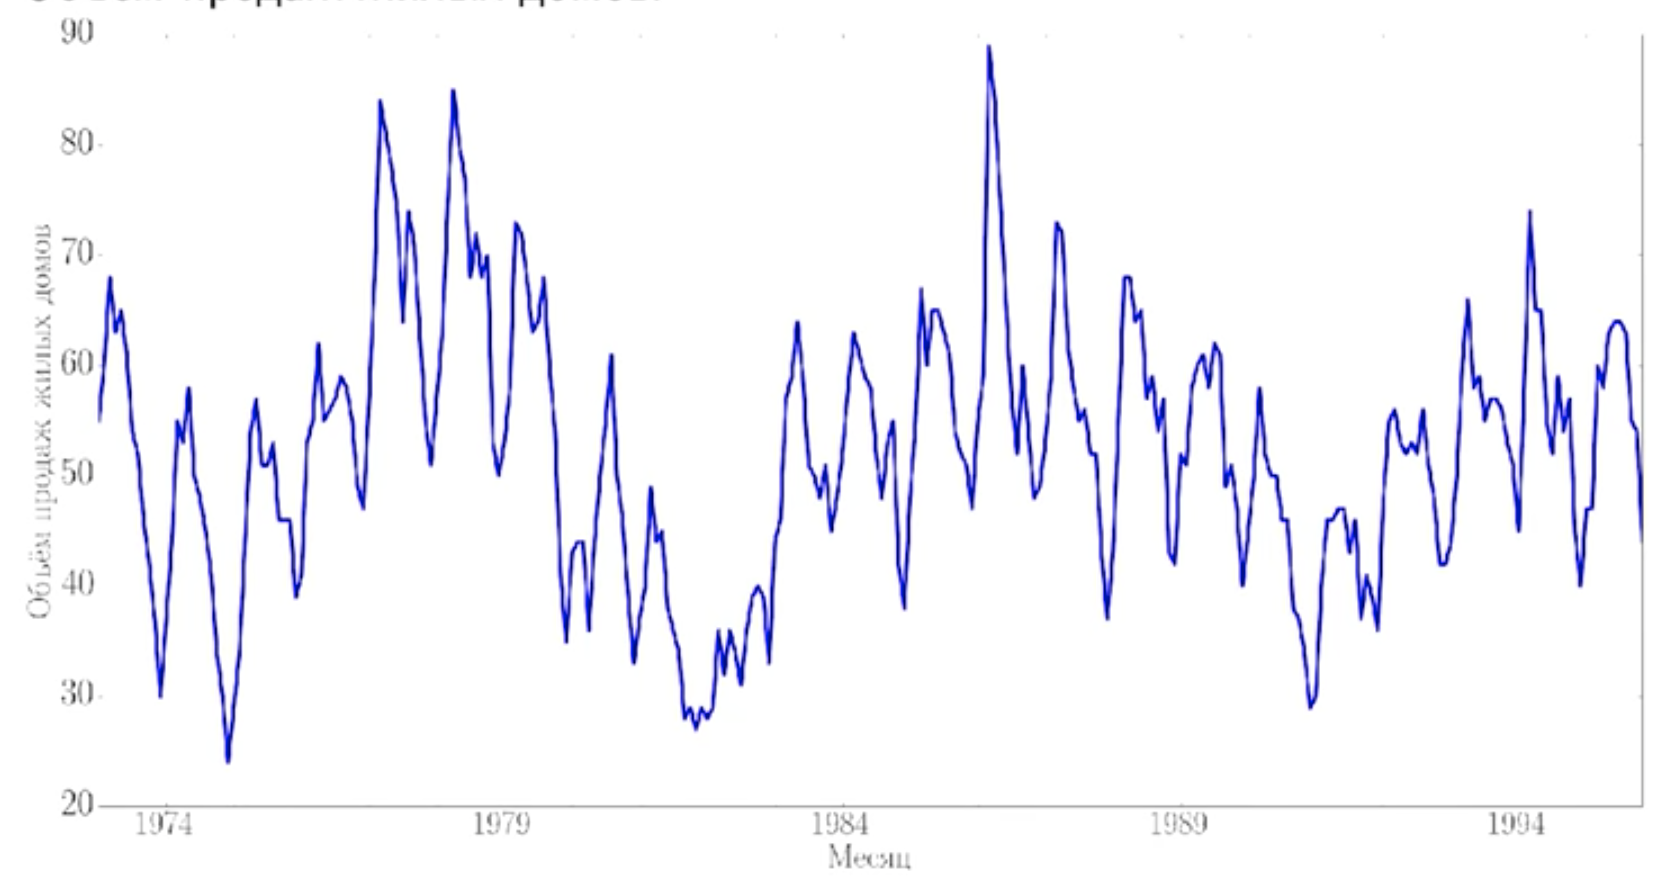
\includegraphics[totalheight=7cm]{main_part/house-sells.png}
% % 	\caption{Объём продажи жилых домов в США}
% % 	\label{sec:purpose:house-sells}
% % \end{figure}

% % На данном графике можно заметить годовую сезонность, длиной премерно равной году, и экономические циклы, которые можно отметить спадами и подъёмами объёмов продаж с нефиксированной временной длиной.




